\section{相関と補助的重回帰（history）}

\subsection{Pearson 相関（数値・二値）}
図 \ref{fig:corr} は主要な数値・二値列の Pearson 相関を\textbf{下三角のみ}表示したものである（重複セルを避ける）。
強い相関は特徴設計上の\textbf{冗長性}の手がかりとなるが、因果ではない。

\begin{figure}[htbp]
  \centering
  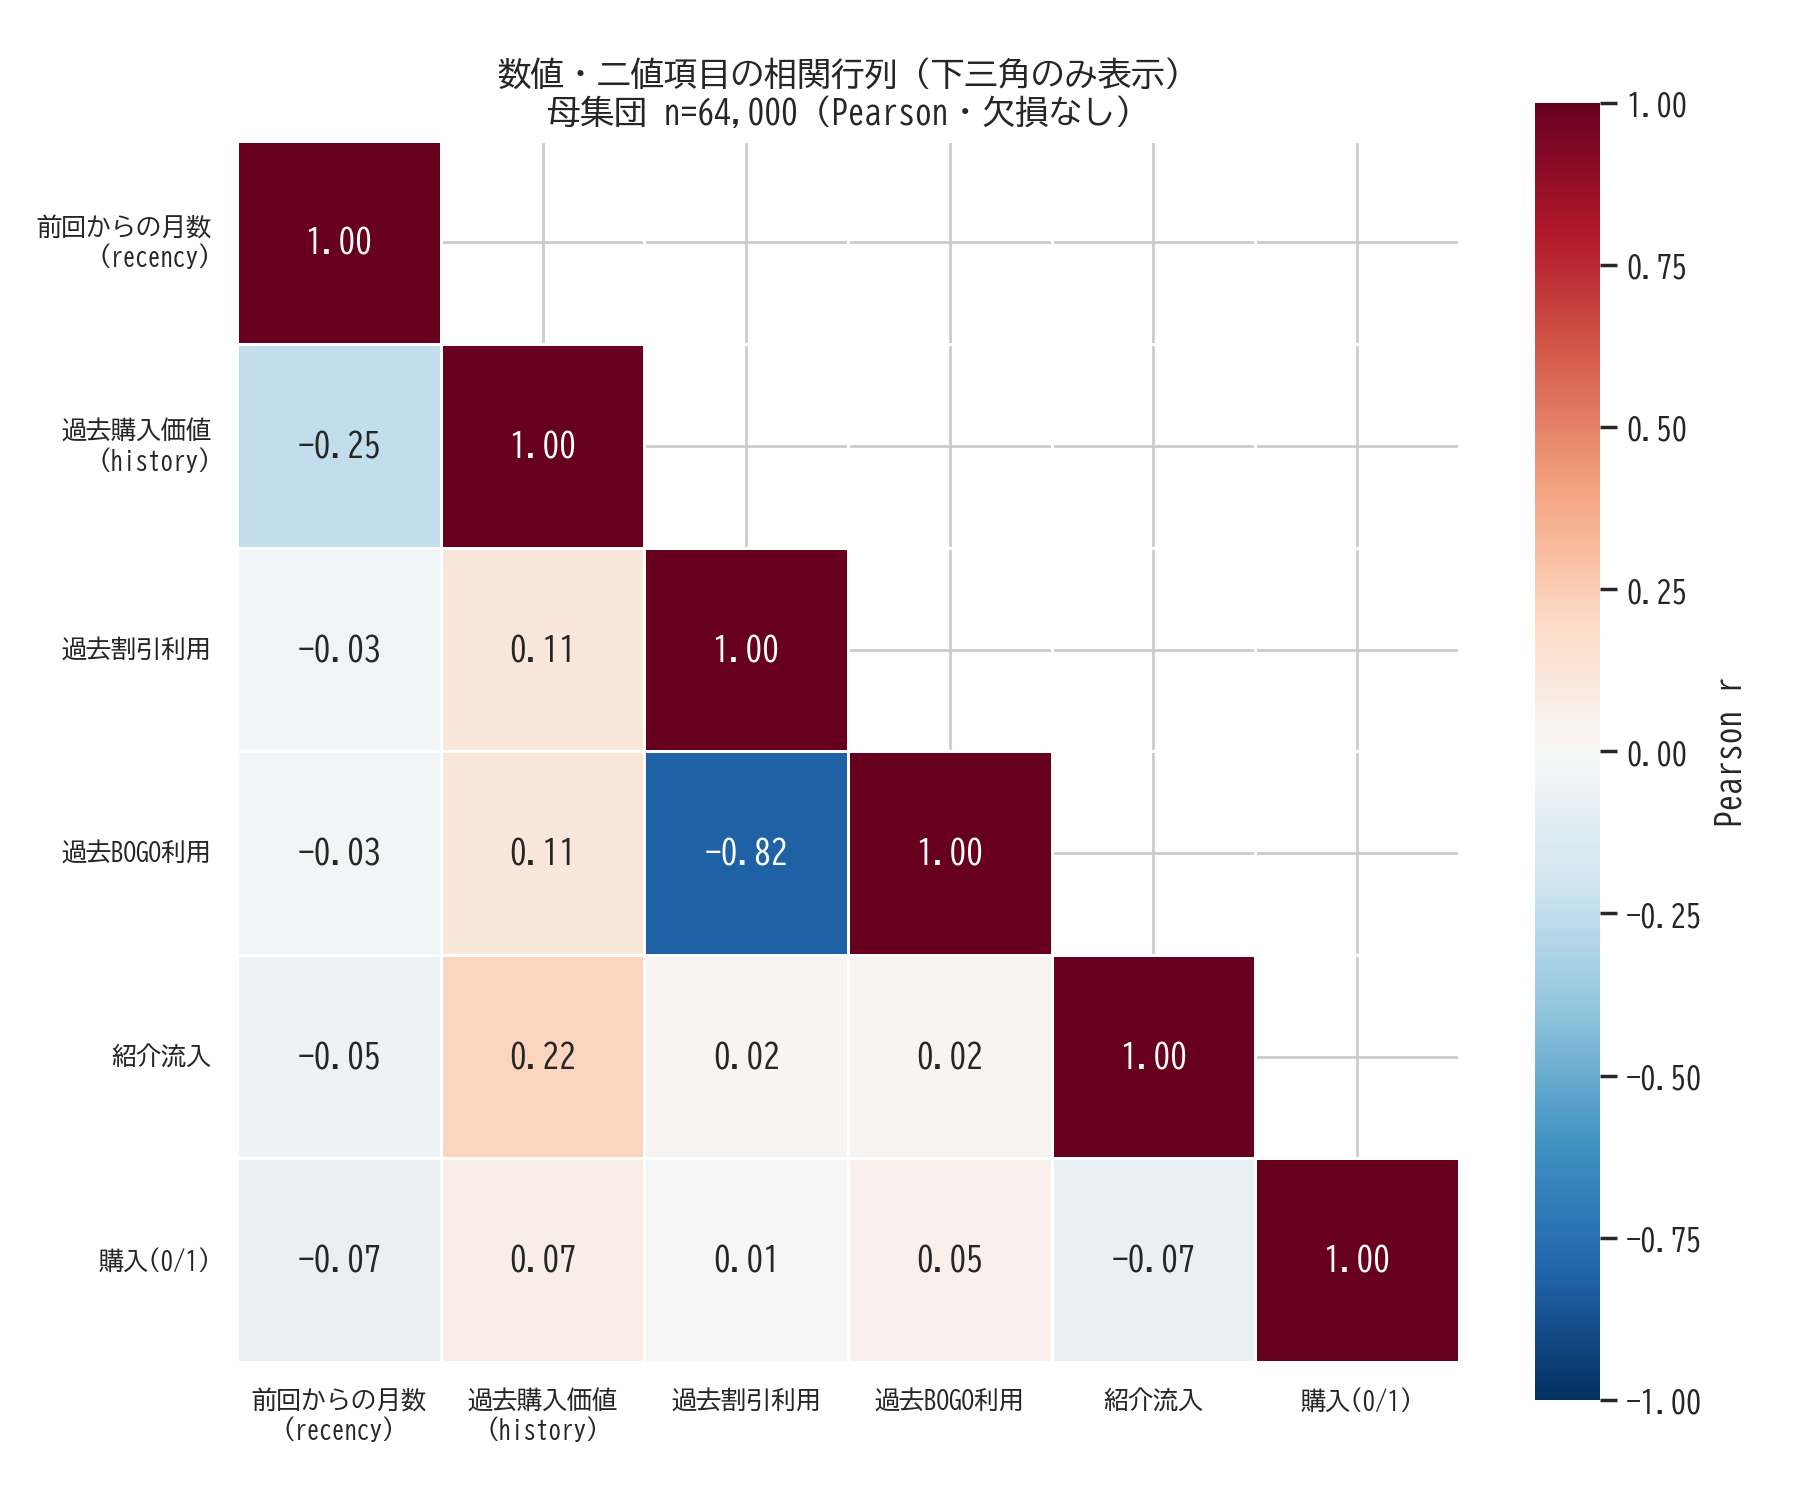
\includegraphics[width=0.92\linewidth]{../figures/improvements/corr_numeric_detailed.png}
  \caption{相関行列（Pearson、下三角）}
  \label{fig:corr}
\end{figure}

\begin{figure}[htbp]
  \centering
  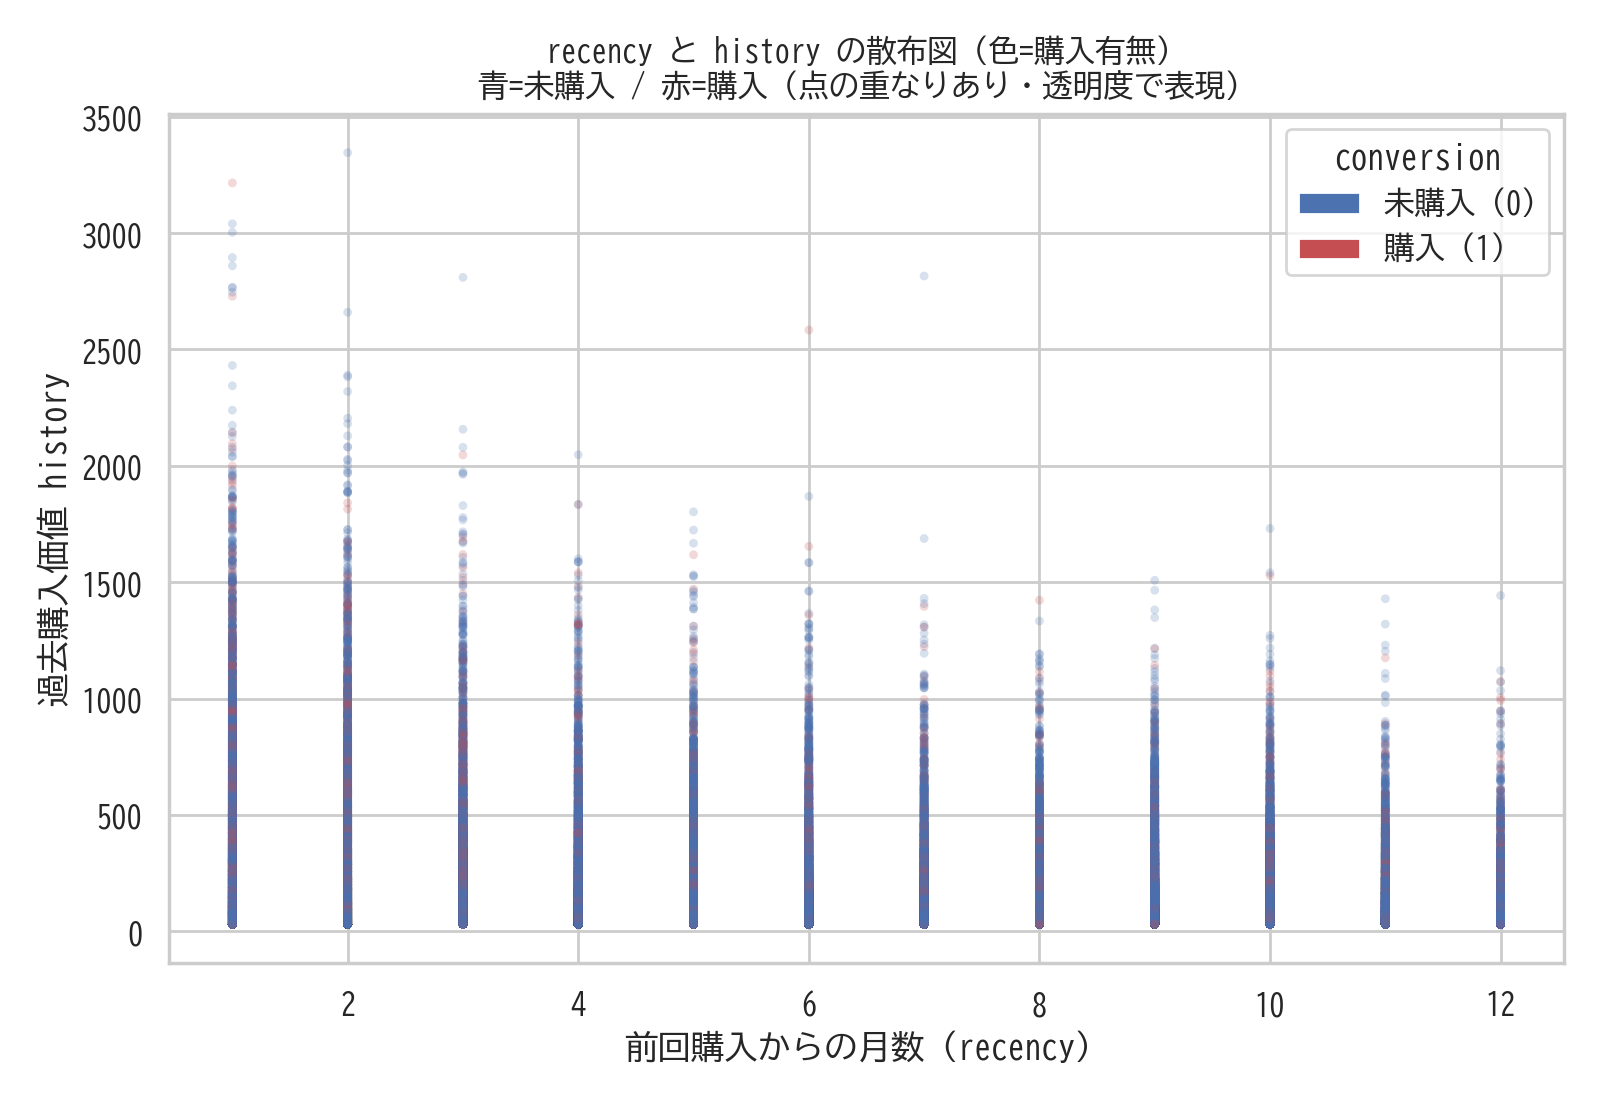
\includegraphics[width=0.88\linewidth]{../figures/improvements/scatter_recency_history_by_conversion.png}
  \caption{recency と history の散布図（色は購入有無）}
  \label{fig:scatter_rh}
\end{figure}

\subsection{OLS（目的変数を history）}
演習で例示される重回帰に対応するため、連続の \texttt{history} を目的変数とした OLS（説明変数は \texttt{recency}, \texttt{used\_discount}, \texttt{used\_bogo}, \texttt{is\_referral}、ロバスト分散 HC1）を付す。
購入予測そのものは次節以降のロジスティック回帰が主である。係数表は \texttt{artifacts/ols\_history\_coefficients.csv}。

\begin{figure}[htbp]
  \centering
  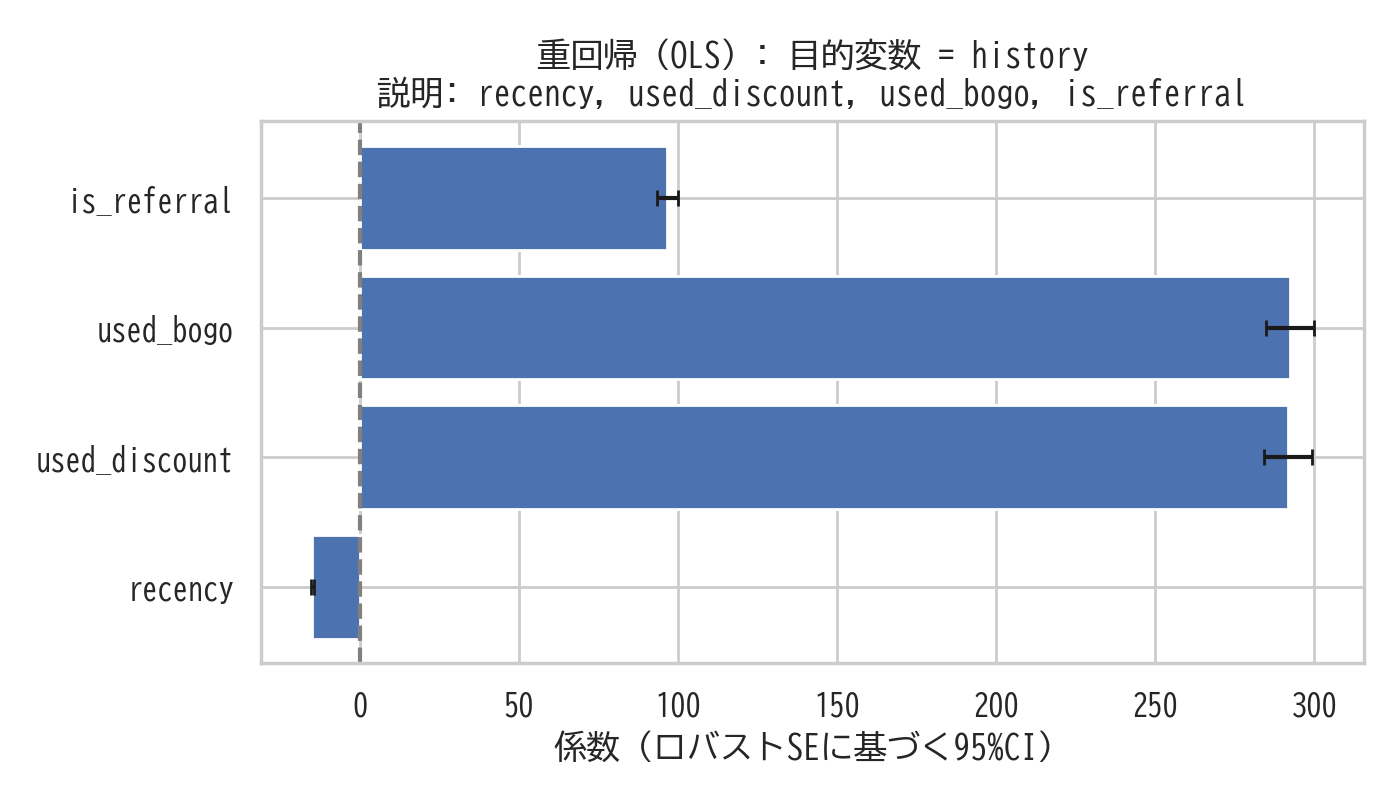
\includegraphics[width=0.78\linewidth]{../figures/improvements/ols_history_coefficients.png}
  \caption{OLS 係数と 95\% 信頼区間（history を目的変数）}
  \label{fig:ols_hist}
\end{figure}

\section{LSI類似表現と分類アブレーション}

各行を英語テンプレの短文に変換し、\textbf{訓練標本のみ}に fit した TF-IDF と TruncatedSVD（次元は \texttt{artifacts/lsi\_tfidf\_diag.json}）を特徴に連結し、
ロジスティック回帰のホールドアウト性能を \textbf{BASE のみ} と比較する（外部 API 不要）。
図 \ref{fig:lsi_ab} は同一分割における AUC / Brier / AP / TopK\% CVR の対比である。

\begin{figure}[htbp]
  \centering
  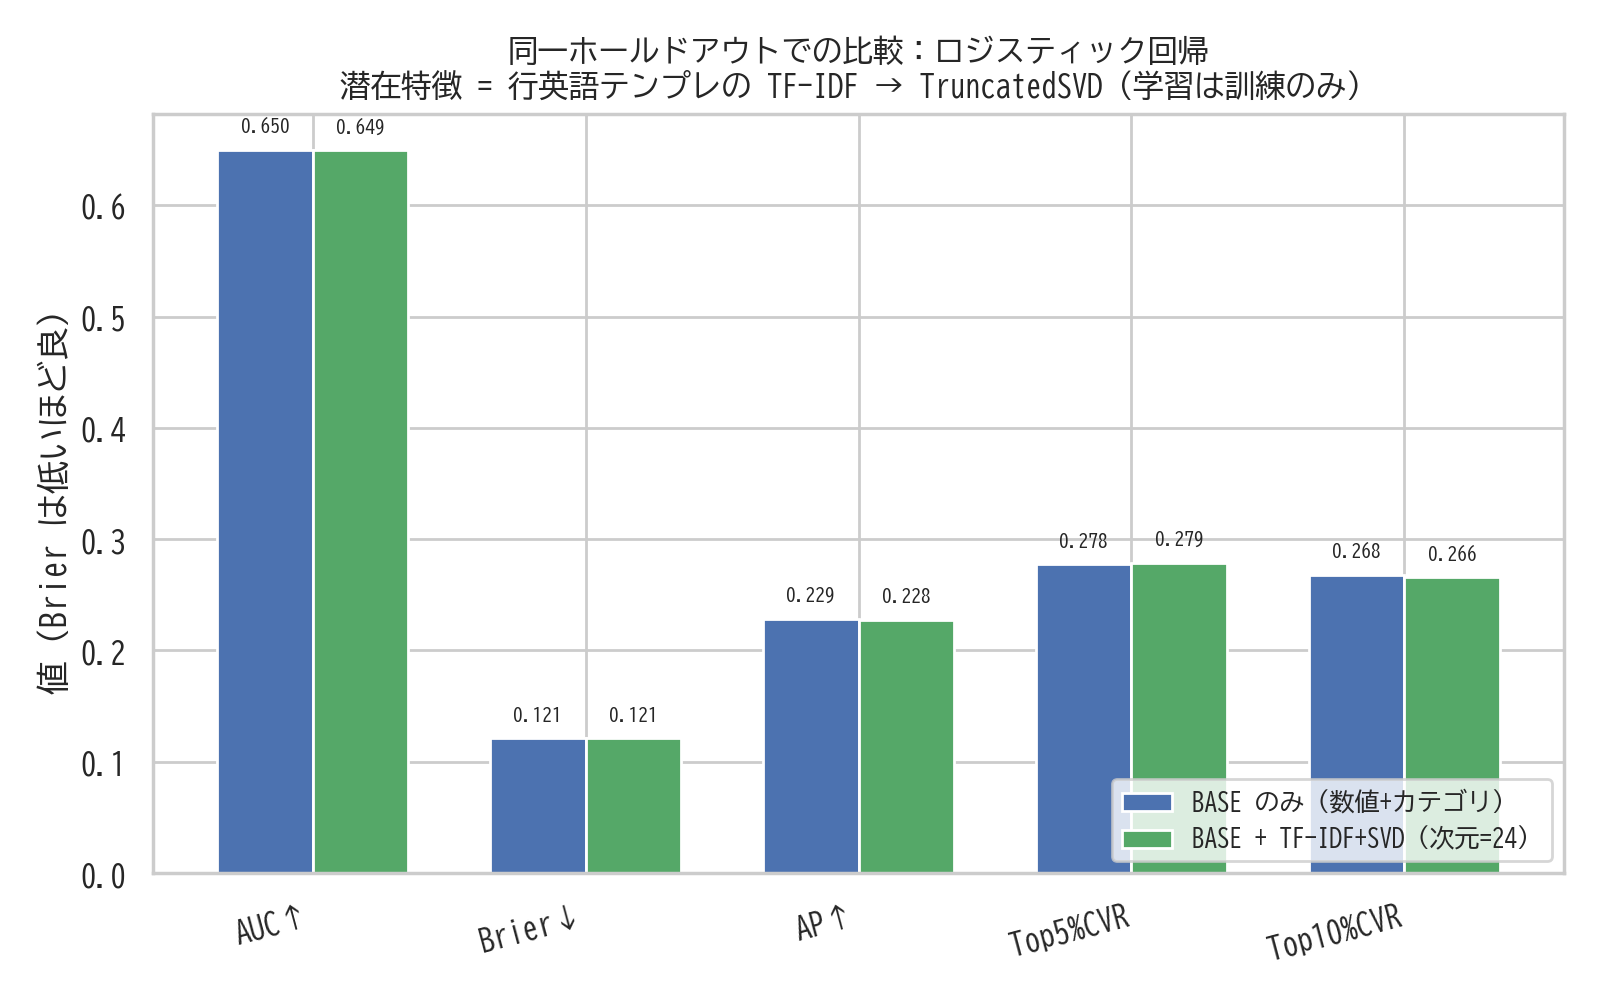
\includegraphics[width=0.92\linewidth]{../figures/improvements/ablation_base_vs_lsi_logreg.png}
  \caption{BASE vs BASE+TF-IDF+SVD（同一ホールドアウト・値ラベル付き棒）}
  \label{fig:lsi_ab}
\end{figure}
